\section{Das Perceptron}
Zu Beginn steht das Perceptron. Es wird hier wie in Abbildung \ref{fig:04_perceptron} veranschaulicht.
Es besteht aus der Summe mehrerer gewichteter Eingabewerte wie auch einem Bias, welcher
die Schwelle einer Aktivierung verschiebt. Die Gewichte werden mit $w_i$, die Eingabewerte mit $x_i$ bezeichnet.
Diese Summe, im folgenden als $net$ bezeichnet, wird in eine Aktivierungsfunktion,
hier eine Sigmoide, gegeben. Der resultierende Wert wird als $z$ bezeichnet. Der Bias hat den fixen Inputwert $-1$,
er wird wiederum über ein Gewicht $w_0$ trainiert/eingestellt.

\begin{figure}[h!]
    \begin{center}
        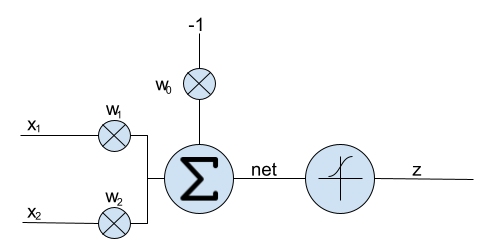
\includegraphics[width=0.6\linewidth]{../common/01_perceptron/00_resources/00_perceptron.png}
    \end{center}
    \caption{Das Perceptron}
    \label{fig:04_perceptron}
\end{figure}

Am Ende dieses Perceptrons steht die Berechnung eines Fehlers. An dieser Stelle wird die quadratische Distanz gewählt.
Man berechnet also die quadratische Differenz zwischen dem erwarteten Wert $d$ sowie dem effektiven Wert $z$.
\begin{align}
    P_{err} = \sum_i^n(d_i - z_i)^2
\end{align}
Im Falle des Perceptrons gibt es nur einen Output-Wert. Daher lässt sich die Fehlerfunktion wie in \ref{eq:01_fehlerfunktion_perceptron}
darstellen.
\begin{align}
    P_{err} = (d - z)^2\label{eq:01_fehlerfunktion_perceptron}
\end{align}

\subsection{Lernverfahren}
Um nun die Gewichte entsprechend ihrem Anteil am Fehler zu korrigieren, wird das Gradientenabstiegsverfahren\footnote{Siehe Kapitel \ref{chapter:01_gradientenabstiegsverfahren}}
verwendet. Dazu muss die Ableitung der Fehlerfunktion bekannt sein. Um diese Ableitung nun einfacher zu gestalten,
wird die Fehlerfunktion mit einem konstanten Faktor $\frac{1}{2}$ multipliziert. Dieser Faktor hat keinen Einfluss
auf Minima oder Maxima, da er an jedem Punkt der Funktion angewendet wird.
\begin{align}
    P_{err} = \frac{1}{2} \cdot (d - z)^2
\end{align}
Nun hat eine Maximierung ebenfalls einen vereinfachenden Vorteil aufgrund der Kettenregel bei der Ableitungsbildung,
weswegen die Fehlerfunktion gedreht wird. Es ergibt sich die endgültige Fehlerfunktion.
\begin{align}
    P_{err} = -\frac{1}{2} \cdot (d - z)^2
\end{align}
Entsprechend lautet die Ableitung unter Anwendung der Kettenregel:
\begin{align}
    \frac{\delta P_{err}}{\delta z} = - \frac{1}{2} \cdot 2 \cdot (d - z) \cdot -1\\
    \frac{\delta P_{err}}{\delta z} = (d - z)
\end{align}

Die Gewichte können anhand des Gradienten korrigiert werden.
\begin{align}
    \begin{pmatrix}w_{0, neu} & w_{1, neu} & w_{2, neu}\end{pmatrix} = \begin{pmatrix}w_{0, alt} & w_{1, alt} & w_{2, alt}\end{pmatrix} + \lambda \cdot \vec{\nabla}
\end{align}
Dieser Gradient setzt sich nun aus der Ableitungskette der verschiedenen Funktionen zusammen, welche nacheinander aufgerufen
und jeweils als Input für die nächste dienen. Dazu wird das Perceptron aus Abbildung \ref{fig:04_perceptron} von
hinten her aufgerollt. Der Gradient lautet demnach:
\begin{align}
    \vec{\nabla} = \begin{pmatrix}\frac{\delta P_{err}}{\delta w_0} & \frac{\delta P_{err}}{\delta w_1} & \frac{\delta P_{err}}{\delta w_2} \end{pmatrix}
\end{align}
An dieser Stelle wird nun die Ableitungskette für $w_0$ näher erläutert. In einem ersten Schritt muss also die
Ableitung der Fehlerfunktion nach $w_0$ gebildet werden. Wie bereits erwähnt, werden die Funktionen nacheinander
aufgerufen und dienen sich gegenseitig als Input. Von hinten her aufgerollt lautet die Aufrufreihenfolge:
\begin{align}
    P_{err} = (d - z(net(w_0, w_1, w_2)))
\end{align}
Für $z$ und $net$ gilt:
\begin{align}
    z = \frac{1}{1 + e^{-net}}\\
    net = -1 \cdot w_0 + x_1 \cdot w_1 + x_2 \cdot w_2
\end{align}

Um nun den Wert des Gradienten für $w_0$ zu bilden, muss die Funktion $P_{err}$ für $w_0$ partiell abgeleitet
werden. Dies geschieht durch konsequentes Anwenden der Kettenregel.
\begin{align}
    \frac{\delta P_{err}}{\delta z(w_0)} = (d - z)\\
    \frac{\delta z(w_0)}{\delta net(w_0)} = z (1 - z)\\
    \frac{\delta net(w_0)}{\delta w_0} = -1
\end{align}

Die gesamte Ableitungskette nach Anwendung der Kettenregel lautet nun:
\begin{align}
    \frac{\delta P_{err}}{\delta w_0} = \frac{\delta P_{err}}{\delta z(w_0)} \cdot \frac{\delta z(w_0)}{\delta net(w_0)} \cdot \frac{\delta net(w_0)}{\delta w_0}\\
    \frac{\delta P_{err}}{\delta w_0} = (d - z) \cdot z \cdot (1 - z) \cdot -1\label{eq:02_ableitungskette_perceptron}
\end{align}
Mit dem Ausdruck \ref{eq:02_ableitungskette_perceptron} lässt sich das Gewicht $w_0$ in einer Iteration korrigieren.
Dasselbe Verfahren wird für die Gewichte $w_1$ sowie $w_2$ angewendet, es resultiert:
\begin{align}
    \frac{\delta P_{err}}{\delta w_1} = (d - z) \cdot z \cdot (1 - z) \cdot x_1\\
    \frac{\delta P_{err}}{\delta w_2} = (d - z) \cdot z \cdot (1 - z) \cdot x_2
\end{align}

\subsection{Das Problem mit XOR und nichtlinearen Funktionen}